\documentclass[]{article}
\usepackage{graphicx}
\usepackage{float}
\usepackage{indentfirst}
\usepackage{setspace}
\usepackage{hyperref}

\begin{document}

\begin{titlepage}

\begin{flushleft}
Matteo NOTTARIS and Nicolas BOINAY \\
\bigskip
Tutor : Maria ZULUAGA
\end{flushleft}

\vspace*{\fill}  
\begin{center}  
     {\huge RSI indicator and Machine Learning}\\[30mm]
     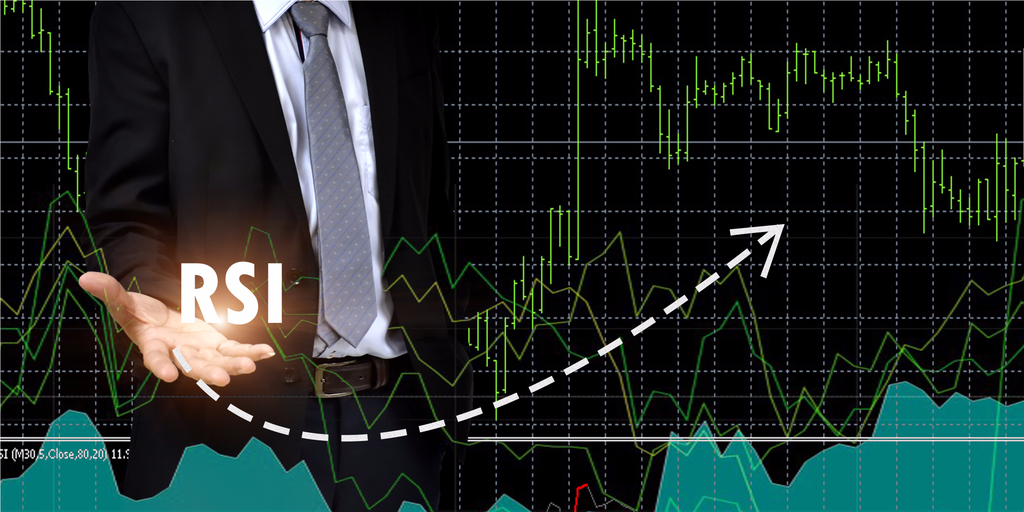
\includegraphics[scale=0.35]{image/rsi_bourse.png}
	 \centering
\end{center}
\vspace*{\fill} 

\end{titlepage}

\doublespacing

\renewcommand*\contentsname{Summary}

\tableofcontents
\clearpage
\singlespacing

\section{Project origin}

\vskip 0.5cm
We wanted to invest ourself in a project linked with finance because we both want to orient our professional careers in this domain.
In order to do so we contacted a FOREX trader working for Crédit Agricole Indosuez Wealth Management, with whom one of us worked during an internship. Our main concern was to find a project's subject usable for traders once finished and with a real application in the trading rooms.

\vskip 0.5cm
We knew that there were already several projects on internet about trying to determine the future evolution of stocks using Machine Learning algorithms. Nevertheless, we wanted for our first ever project in the subject to try something new, ambitious and above all interesting for traders. Therefore, our contact told us to work on financial indicators which are helping traders to interpret trends on the market.

\vskip 0.5cm 
At the beginning, the idea was to write algorithms capable of determining for a given representation of the market the most relevant indicator. Therefore, traders would just need to see which indicator is returned by algorithms and use it in order to interpret a situation. However, we soon understood that it was maybe a bit too complex for beginners especially with the time we had to develop our project.
Therefore, we slightly changed the project to have it as it is today.

\section{Project description}

\vskip 0.5cm
As explained above the project definition slightly changed from our original thoughts. We focus on one commonly used indicator for traders which is called RSI for Relative Strength Index. RSI is an indicator which gives an indication on the trend of an asset, using two different parameters, which we will call the upper and the lower one. If the RSI signal is over the upper parameter it means that the asset we are interested in (EURUSD in our case) is overbought and therefore there will probably have a reversal in the asset trend. Hence the RSI tells us to sell the asset if the price is high and rebuy it after the reversal, this would allow us to make a profit. The lower parameter is working exactly the same, because when the RSI signal is under it the asset is over sold and the asset trend might go up strongly. As a result the RSI tells us to buy while it is low and sold after the reversal.

\vskip 0.5cm
However, the main problem with this indicator is that it is always used with two parameters, RSI(80,20) or RSI(70,30) for instance. We thought that depending on the market situation those two parameters could be adapted  for the RSI to be even more precised. 

\vskip 0.5cm
There were three main steps in order to lead this project to its end.\\
The first was to determine what could be a representative picture of a market and then extract all the data sets corresponding.\\
The second one was to find which couple of parameters suits the best for a given situation.\\
With this second step we were able to develop a new data set used for the third and last step of the project which is the training of a Neural Network in order to find the regression function suiting best our problem.  

\section{Extraction of the data sets}

\vskip 0.5cm
For the sake of our project we needed to extract a lot of different data sets (Annexe 1) in order to perfectly determine what represents a market situation. To do so we contacted our trader colleague who was far more capable than us to do this list of important representant of the market.\\
We used two different websites to extract the data sets.\\
The first one was \href{https://www.alphavantage.co/}{AlphaVantage} in order to extract the RSI signal for our asset : the dual currency EUR/USD.
The second website we used, in order to download the data from all the other stocks, was \href{https://fr.finance.yahoo.com/}{Yahoo Finances}. 

\vskip 0.5cm
The hard part in it wasn't downloading the data sets from the websites and loading them in excel files, but it was succeeding on making sure that all of them were over the same dates set. Indeed, we needed to be sure that we had the value of each indicators for a given date. We succeeded in doing so, using the manipulation of Python's dictionnaries and arrays.At the end of this step we had more than 2900 common and different dates for all the data set. We could now use this data set as we wanted.

\section{Creation of a new data set}

\vskip 0.5cm
The second step of the project was to generate, using the data sets downloaded and shaped in the first step, a new data set which would contain, for different couple of parameters, the most relevant market situation.

\vskip 0.5cm
In order to do so we had to determine how to estimate the best situation according to a couple of parameters. We decided, with the trader, that the best way was to calculate a performance using the RSI signal and the two chosen parameters. Concretely, we put ourselves in a situation of having a certain amount of money on day 0 and then we follow exactly the instructions of the \(RSI(p_1,p_2)\) which means that if it tells us to sell we do so and same if it tells us to buy. Then we calculate a performance, in other words we calculate our benefits in percentage, compared to the situation where we would have not listened to it.\\
At the end we look for this given couple of parameters which of the 2900 dates has the highest performance. We did that for every parameter from RSI(90,10) to RSI(51,49) incremented by 0.5 each time. For these 80 different couples we attribute 10 different dates which correspond to the 10 best performances. 

\vskip 0.5cm
This new data set will be used in order to train our Neural Network in the next step of the project. 

\begin{figure}[hbt!]
	\center{}
	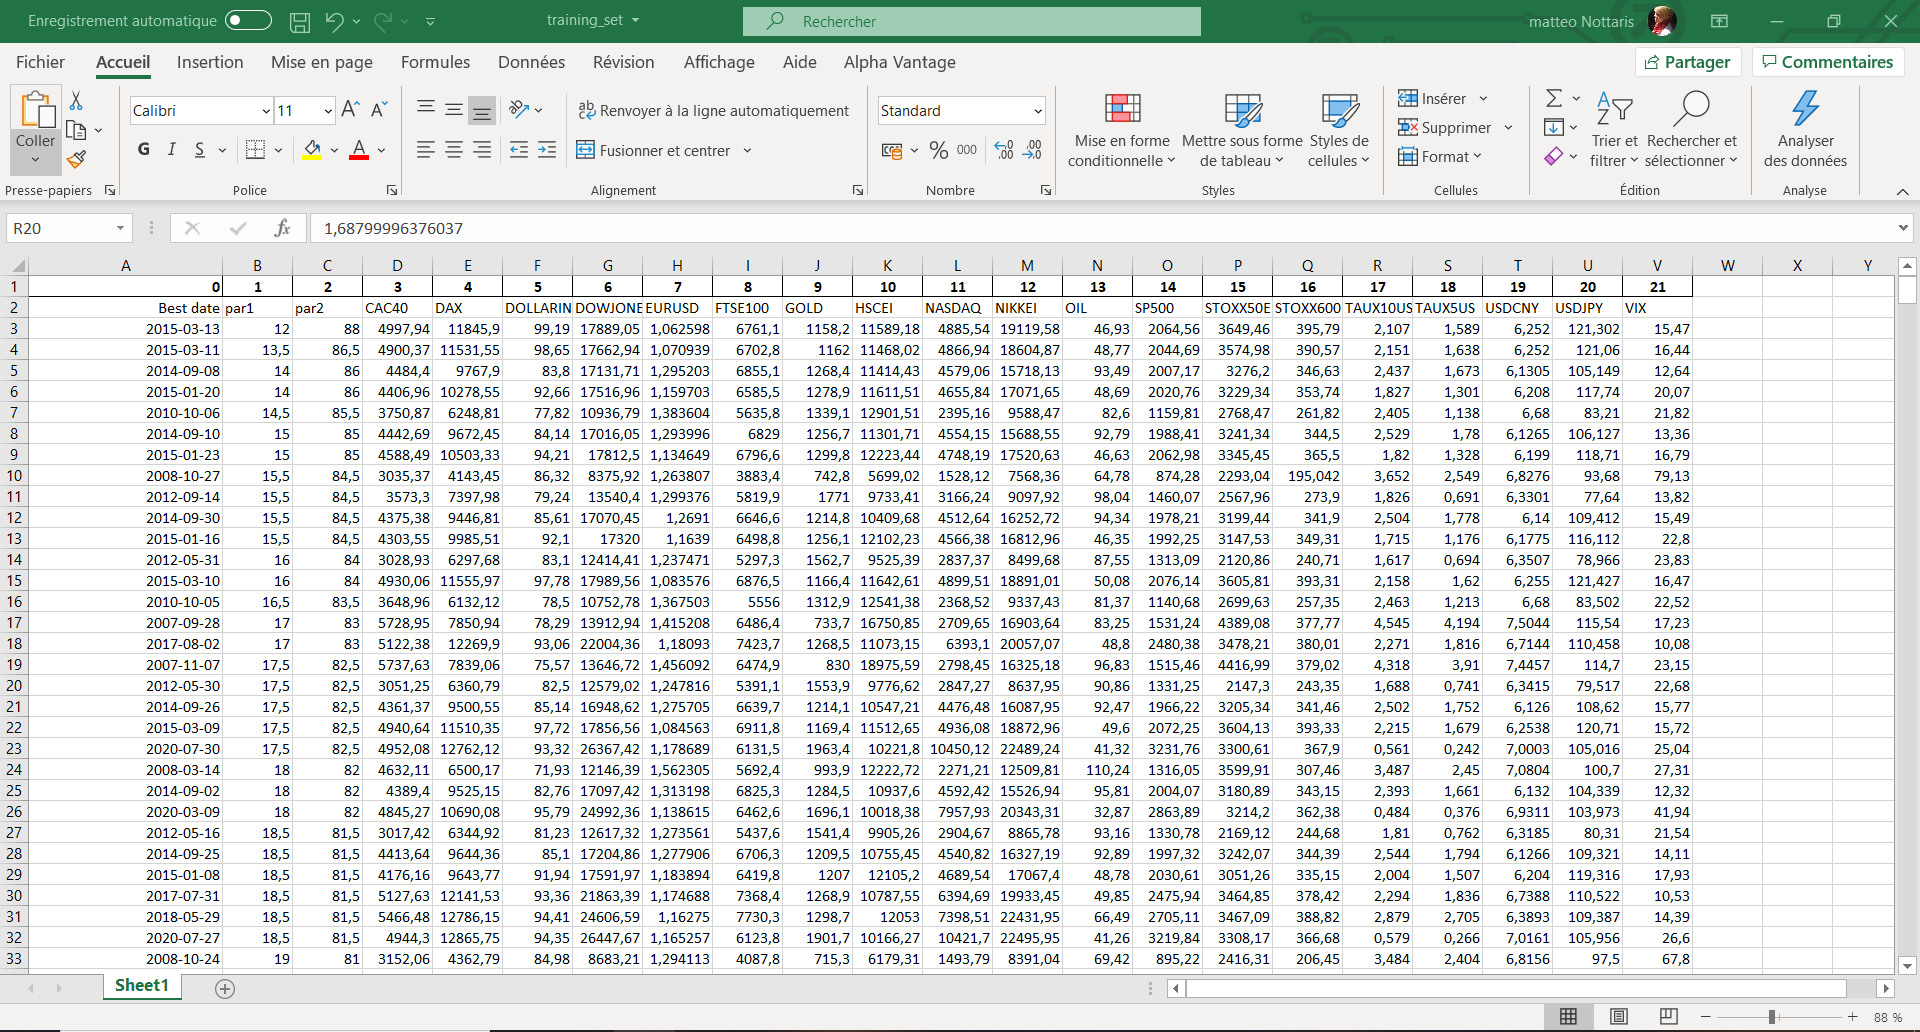
\includegraphics[scale=0.35]{image/training_set.png}
	\caption{New, neural network's training data set}
\end{figure}


\section{Use of a Neural Network}
\subsection{Initial thoughts}
\vskip 0.5cm
In this last step of the project we are trying to train a neural network. This neural network takes as inputs a vector of shape (19,1), corresponding to all the market indicators used to define a market situation (see Annexe 1). As output the neural network sends back a vector of shape (1,1) corresponding to the first optimal parameter which should be used considering the situation in input. The second parameter can be easily determined : \[par_{1} + par_{2} = 100\].
\vskip 0.5cm
In order to do so, we took an already implemented neural network that we used during one of our previous labs in class, and tried to adapt it to our situation. \\
The first main difference between the neural network problem in the lab session and our project is that the problem we are tackeling is a regression problem while the other one was a classification exercise. We understood that when we found odd results especially between 0 and 1 due to the sigmoid activation function used.

\vskip 0.5cm
As we understood that our problem is a regression one, we changed the activation function on the last layer of our network by a regression function. However, we kept struggling  with this neural network, and our tutor wisely advised us to use a python library like scikit-learn to implement it, because this new network might be more robust.

\subsection{Scikit-Learn}
\vskip 0.5cm
The use of scikit-learn was very helpful because we just had to focus on the choice of parameters and not anymore on the concrete development of the neural network.\\
Our subject was a regression problem, therefore we compared four different linear functions : \textit{tanh}, \textit{identity}, \textit{logistic} and \textit{relu}.
For each of those ones we used a function of scikit-learn called \textit{GridSearchCV}, in order to find the optimal parameters. \\
However, even with the help of those tools the results were very disappointing. The main issue was that our output vector was composed of only one value, which we assimilated to a sort of average of all supposed output value. We understood that this issue was generated because our outputs of our $y_{train}$ were too close from each other no matter how different were the inputs. Then it would just generate an average of our $y_{train}$ values which is not what we wanted to get an efficient and precise output.  Indeed we realized that the \(w_{i}\) must be close to 0. Therefore, in the prediction formula, the neural network was only returning the constant \(w_{0}\) in : \(y_{pred} = w_{0} + \sum w_{i}*x_{i}\).\\)

In order to tackle this issue, we decided to make sure to spread the \(y_{train}\) values before training the neural network. We used different functions to spread the data, but the most efficient one was to multiply by 1000 and then divide by 1000 at the end of the neural network. Nevertheless, the results were not as expected. The Mean-Squared-Error (MSE) didn't decrease by a lot but for two functions (\textit{relu} and \textit{identity}), the outputs vectors weren't composed of a single value anymore. The neural network was actually working and trying for each different input to predict a coherent output.\\
We were not yet satisfied by the results, and we thought that we could reduce our dataset and only keep the most efficient market situation for each couple of parameter. As a result we trained our neural network with around 70 lines of data instead of 700, and this had a major effect on the result. First of all we saw the MSE decreasing for every functions. Secondly, now the \textit{tanh} function was, as \textit{relu} and \textit{identity}, working as expected and returning different outputs for various inputs. \\
Overall, we can see in the following table that the results are far better when the dataset is smaller, which probably shedlight a problem of overfitting in the first case. Moreover, the best function in order to tackle our problem is \textit{tanh} because it shows the smallest MSE.\\

\begin{figure}[hbt!]
	\center{}
	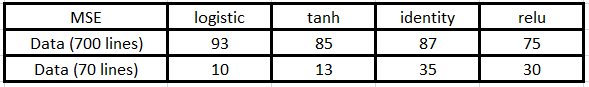
\includegraphics[scale=0.8]{image/results.png}
	\caption{MSE for different functions and datasets}
\end{figure}


\section{What should be improved}
\vskip 0.5cm
This project was very interesting, especially for beginners  in machine learning like us. Obviously, the results we got could be much better and there are two main reasons for it. \\
The first one is that the data we are looking at could be wider.Indeed, we could try to find better situations for the different couples of parameters. For example looking for datas from previous years. We could even look for the market situation every hours, instead of everyday, to increase the number of potential situation to optimally fit the given parameters. \\
The second reason is that maybe neural networks from scikit-learn are not powerful or robust enough. As a result by using stronger neural networks we could obtain far better results for some of the functions like \textit{tanh} or \textit{relu}. \\
Overall, this study is primary and there is still a lot of work to improve it.


\section{Sharing of the work}

\vskip 0.5cm
For the beginning of the project we spread the work pretty evenly.
Nicolas did most of the extraction of data from the two websites (AlphaVantage and Yahoo Finance). 
Then Matteo did the shaping of the data and the creation of the new data set.\\
Concerning the last part, the use of neural network, we shared the work in two and each of us was trying some set of parameters different application functions to find the most suitable situation to our problem.

\section{Annexe}
\subsection{Annexe 1} 
\begin{figure}[hbt!]
	\center{}
	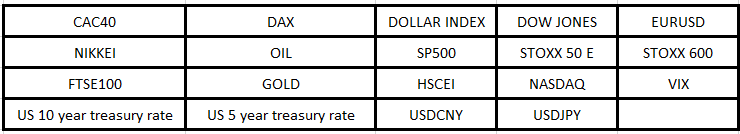
\includegraphics[scale=0.5]{image/marketSituation.png}
	\caption{All market indicators used in our case}
\end{figure}

\end{document}
